\documentclass[toc]{beamer}
\usepackage[ngerman]{babel}
\usepackage{comment}
\usepackage{nameref}
\usepackage[official]{eurosym}

\usetheme{Warsaw}
\usecolortheme{seahorse}



\title{Entwicklung eines Moduls zur Umstellung von direkten Datenbankzugriffen zu einer gekapselten Datenbankkommunikation mit optionaler Simulationsmöglichkeit}
\author{Frank Loleit}
\institute{Fachinformatiker (Anwendungsentwicklung)}
\titlegraphic{
\includegraphics[scale=0.2]{argusLogo.png}}
\date{\today}






\defbeamertemplate*{footline}{infolines theme}
{
  \leavevmode%
  \hbox{%
  \begin{beamercolorbox}[wd=.333333\paperwidth,ht=2.25ex,dp=1ex,center]{author in head/foot}%
    \usebeamerfont{author in head/foot}\insertshortauthor%~~(\insertshortinstitute)
  \end{beamercolorbox}%
  \begin{beamercolorbox}[wd=.333333\paperwidth,ht=2.25ex,dp=1ex,center]{title in head/foot}%
    \usebeamerfont{title in head/foot}Argus Data Insights
  \end{beamercolorbox}%
  \begin{beamercolorbox}[wd=.333333\paperwidth,ht=2.25ex,dp=1ex,right]{date in head/foot}%
    \usebeamerfont{date in head/foot}\insertshortdate{}\hspace*{2em}
    \insertframenumber{} / \inserttotalframenumber\hspace*{2ex}
  \end{beamercolorbox}}%
  \vskip0pt%
}



\setbeamertemplate{blocks}[rounded][shadow=false]
\setbeamercolor{block body}{bg=white}
\setbeamercolor{block title}{bg=white, fg=blue}

\makeatletter
\newcommand*{\currentname}{\@currentlabelname}
\makeatother


\begin{document}




\begin{frame}
\titlepage
\end{frame}

\begin{frame}
    \frametitle{Inhalt}
    \tableofcontents
\end{frame}

\section{Einleitung}
    \subsection{Herangehensweise}
        \begin{frame}{Ausgangsüberlegung}
            \begin{block}{Customer Obsession}
                    Wirtschaftsphilosophie, die den Kunden als Maßstab für alle Überlegungen
                    des ökonomischen Denkens und Handels emporhebt. Gemäß dieses Ansatzes gibt es keine den Wünschen des Kunden übergeordneten Maxime.
            \end{block}
        \end{frame}
        
    \subsection{Projektbeschreibung}
        \begin{frame}{Grundlegen Ziele des Projekts}
        %Hier können grob zwei Säulen unterschieden werden:
                \begin{columns}
                    \column{0.5\textwidth}
                        \begin{block}{1. Query-Tracing}
                            Es muss möglich sein, Queries zurückzuhalten, um nicht Gefahr zu laufen, Kundendaten zu verändern. Eine detaillierte Rückmeldung über die Query muss ausgegeben werden.
                        \end{block}
                    \column{0.5\textwidth}
                        \begin{block}{2. Command-Generator}
                            In Zukunft sollen Objekte der .NET-Klasse \glqq SqlCommand\grqq{} automatisch auf Basis von Table-Models generiert werden. Das schließt auch das Generieren von Queries mit ein.
                        \end{block}
                \end{columns}
        \end{frame}

    \subsection{Das Unternehmen}
        \begin{frame}{Das Unternehmen Argus Data Insights}
            \begin{figure}[htp]
                \centering
                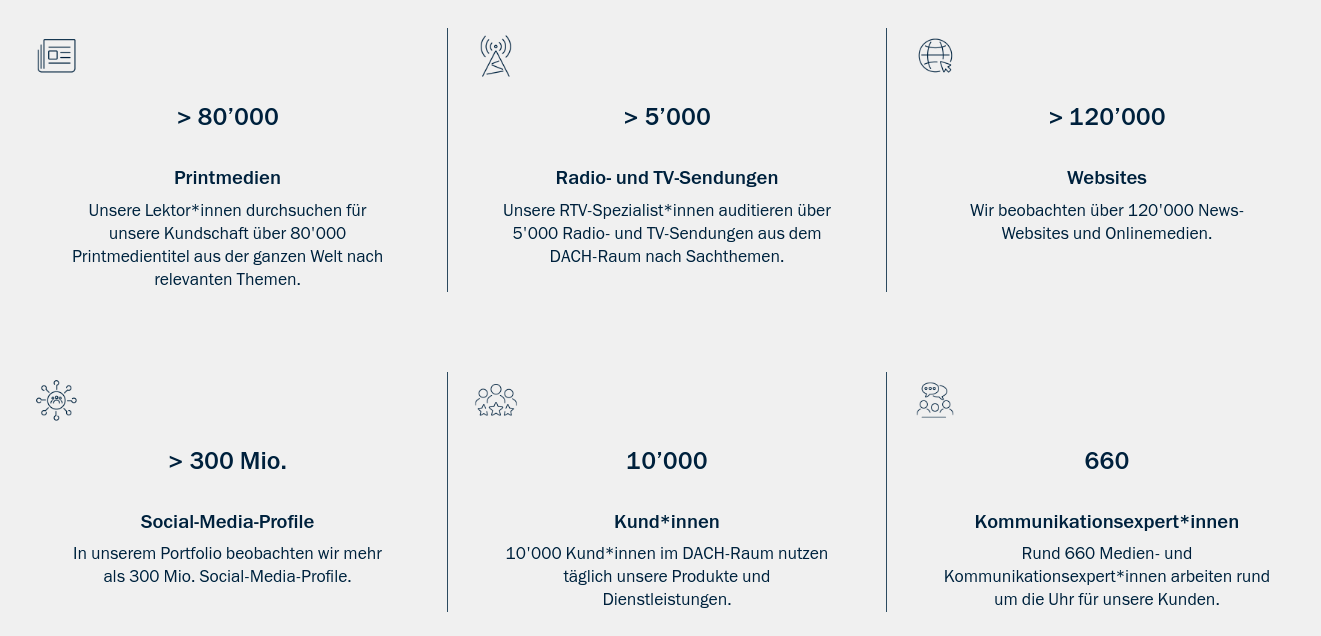
\includegraphics[scale=0.23]{ArgusProfil.png}
                \caption{Portfolio}
            \end{figure}
        \end{frame} 
        
        \begin{frame}{Das Unternehmen Argus Data Insights}
            Argus existiert seit über 125 Jahren. Die Ausrichtung der Arbeit auf Datenbanken und Softwareprodukten begann vor rund 25 Jahren:
            \begin{figure}[htp]
                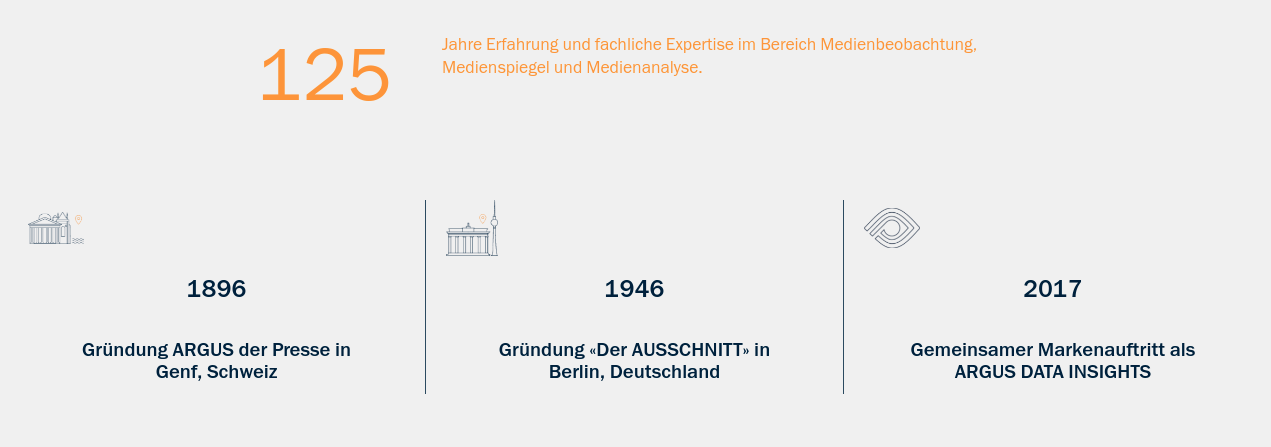
\includegraphics[width=\textwidth]{argusGeschichte.png}
                \caption{Geschichte}
            \end{figure}
        \end{frame}   
        
        \begin{frame}{Desktop-Applikation \glqq Arche\grqq{}}
            \begin{columns}
            \column{0.5\textwidth}
                \begin{figure}[htp]
                                \centering
                                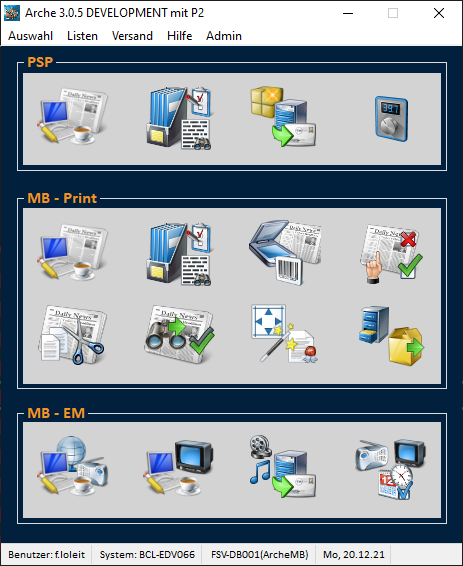
\includegraphics[scale=0.4]{arche.png}
                                \caption{Startbildschirm}
                                \label{fig:my_label}
                            \end{figure}
                \column{0.5\textwidth}
                Die Desktop-Applikation \glqq Arche\grqq{} dient der Beschaffung, Verwaltung und Aufbereitung von Print-, Online- und Rundfunkmedien.
            \end{columns}
        \end{frame}
        
        \begin{frame}{Technische Rahmendaten}
            \begin{block}{Architektur}
                \glqq Arche\grqq{} ist im .NET-Framework 3.5 geschrieben und verfügt über keine einheitliche Dokumentation. Front- und Backendlogik sind nicht strikt getrennt.
            \end{block}
            \begin{block}{Datenbankkommunikation}
                Um die Kommunikation zwischen .NET und SQL zu gewährleisten, stehen hartkodierte Queries in Persistence-Klassen bereit.
            \end{block}
        \end{frame}
                
    \subsection{Projektbegründung}
        \begin{frame}{Probleme mit manueller Kodierung}
            Bisher müssen .NET-Attribute und Tabellenspalten manuell hinzugefügt werden, was fehleranfällig und zeitaufwändig ist:
            \begin{figure}[htp]
                \centering
                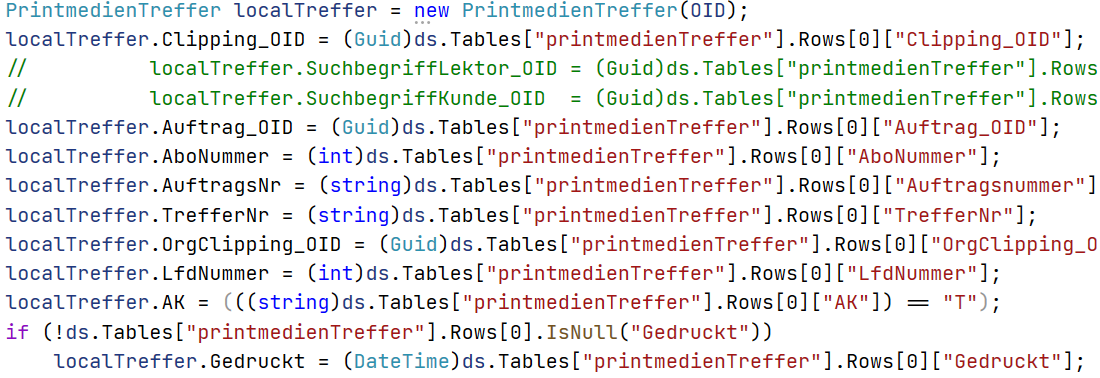
\includegraphics[scale=0.35]{archeChaos.PNG}
                \caption{Legacy-Code}
            \end{figure}
        \end{frame}    

\section{Projektplanung}
    \subsection{Zeitliche Einteilung}
        \begin{frame}{Übersicht der einzelnen Phasen}
            \begin{columns}
                \column{0.6\textwidth}
                    \begin{tabular}{lr}
                    
                    \textbf{Projektphase} 		& \textbf{Geplante Zeit}    \\
                    
                    Analysephase 				& 7 h	 		            \\
                    Entwurfsphase				& 11 h	 		            \\
                    Implementierung      		& 40 h	 		            \\
                    Abnahme             		& 2 h 			            \\
                    Dokumentation               & 10 h 			            \\
                    
                    \textbf{Gesamt}	 			& \textbf{70 h}	            \\
                    \end{tabular}
                \column{0.4\textwidth}
                    Die Implementierung nahm die meiste Zeit in Anspruch. Für die Dokumentation sind Notizen aus den vorigen Phasen mit eingeflossen.
        \end{columns}
    \end{frame}
    

        \begin{frame}{Detaillierte Zeitplanung (1)}
            \begin{table}[ht]

		\begin{tabular}{ l r }
			%\hline
			
			\textbf{Analysephase} 										& \textbf{7 h}	\\
			%\hline			
			\quad 1. Ist-Analyse												& 5 h			\\
			\quad 2. Kostenanalyse            								& 2 h			\\		
			\quad 3. Kommunikation mit dem Fachbereich						& 1 h			\\
			%\hline

			\textbf{Entwurfsphase} 										& \textbf{11 h}	\\
			%\hline
			\quad 1. Datenbanken sichten										& 1 h			\\
			\quad 2. Programmiersprachen und Frameworks auswählen				& 2 h			\\		
			\quad 3. Graphische Benutzeroberfläche skizzieren					& 2 h			\\
			\quad 4. Logik für Table-Models entwerfen						& 3 h			\\
			\quad 5. Konvertierungslogik der Datentypen erarbeiten            & 1.5 h			\\	
			\quad 6. Logiken für SqlCommand-Generierung skizzieren            & 1.5 h			\\	
			%\hline

			

		\end{tabular}
		
\end{table}	
    \end{frame}
            
         \begin{frame}{Detaillierte Zeitplanung (2)}
            \begin{table}[ht]

		\begin{tabular}{ l r }
			\textbf{Implementierungsphase} 								& \textbf{40 h}	\\
			%\hline
			\quad 1. GUI designen										            & 3 h 			\\
			\quad 2. Textformatierung einpflegen							        & 5 h 			\\
			\quad 3. Query-Verarbeitung programmieren 							& 4 h 			\\
			\quad 4. Andockstellen im bestehenden Code identifizieren			    & 2 h 			\\
			\quad 5. QueryRequest-Klasse programmieren							& 6 h 			\\
			\quad 6. Skripte für das Generieren von Table-Models schreiben	& 7 h 			\\
			\quad 7. Query-Generator implementieren                               & 5 h 			\\
			\quad 8. Datenkonvertierung einbinden    						        & 4 h 			\\
			\quad 9. Refoktorierung der bestehenden Datenbanklogik               & 2 h 			\\
			\quad 10. Test der neuen Datenbankkommunikation						& 2 h 			\\			
			%\hline

		

		\end{tabular}
		
\end{table}	
    \end{frame}      
    
\begin{frame}{Detaillierte Zeitplanung (3)}
            \begin{table}[ht]

		\begin{tabular}{ l r }
			

			\textbf{Abnahme und Schulung}		 						& \textbf{2 h}	\\
			%\hline
			\quad 1. Abnahme durch Fachabteilung								& 1 h 			\\
			\quad 2. Installation												& 1 h 			\\
			%\hline

			\textbf{Erstellen der Dokumentation} 						& \textbf{10 h}	\\
			%\hline
			\quad 1. Erstellen der Projektdokumentation						& 8 h 			\\
			\quad 2. Erstellen der Entwicklerdokumentation					& 2 h 			\\
			
			%\hline

			\textbf{Gesamt}	 											& \textbf{70 h}	\\
			%\hline

		\end{tabular}
		\caption{Zeitplan}
\end{table}	
    \end{frame}     
    
\subsection{Auswahl der Ressourcen}
    \begin{frame}{Auswahl der integrierten Entwicklungsumgebung (IDE)}
    Punkte (P), Verteilung (V) und gewichtete Punkte (G):
        \begin{table}[ht]

	%\hline\hline
		\begin{tabular}{|| l | c | c | c | c | c | c | c ||}
	    \hline	
	    
	    \multicolumn{2}{||c|}{} & \multicolumn{2}{|c|}{VS2019}  & \multicolumn{2}{|c|}{Rider}  & \multicolumn{2}{|c||}{MonoDev}   \\
	    \hline
	    Kriterium & P & V & G  & V & G & V & G \\
	    \hline
	    Preis & 20 & 1 & 20 & 2 & 40 & 5 & 100 \\
	    Videos & 10 & 1,75 & 17,5 & 0,25 & 2,5 & 0,1 & 1 \\
	    Foreneinträge & 5 & 1 & 5 & 1 & 5 & 0,1 & 0,5 \\
	    Erlernbarkeit & 15 & 0,25 & 3,75 & 1 & 15 & 3,7 & 55,5 \\
	    Verbreitung & 30 & 4 & 120 & 2 & 60 & 0,1 & 3 \\
	    Features & 20 & 2 & 40 & 3,75 & 75 & 1 & 20 \\
	    \hline
	    Summe & 100 & 10 & \textbf{206,25} & 10 & 197,5 & 10 & 180 \\
	    
		\hline
		
		
	
		
			\end{tabular}
			\caption{IDE Scoring}
			\end{table}
    \end{frame}

\subsection{Kostenübersicht}
    
    \begin{frame}{Personalkosten}
    Bei der Berechnung der Personalkosten wird ein Handlungskostenzuschlag von 30\% angenommen:
\begin{table}
\resizebox{11cm}{!}{
        \begin{tabular}{|| l | l | c | c | c | c | c ||}
	    \hline	
	    
		\textbf{Bei}    &   \textbf{Für}  & \textbf{Std.}  & \textbf{Lohn/Std.}   & \textbf{Lohn} & \textbf{30\%}    &  \textbf{Summe}   \\ 
		\hline
		
		
		Entwickler          & Unterstützung   &	4	& 40,00 €	& 160,00 €	    & 48,00 €	    & 208,00 €\\
		%\hline
		Ausbilder           &	Betreuung  &	8	& 45,00 €	& 360,00 €	    & 108,00 €	    & 468,00 €\\
		%\hline
		Praktikant          &	Durchführung &	70	& 10,00 €	& 700,00 €	    & 210,00 €	    & 910,00 €\\
		%\hline
		PO      &	Kosteninfo           &	2	& 60,00 €	& 120,00 €	    & 36,00 €	    & 156,00 €\\
		\hline%\hline
		Personal            &	                                &	84	& 155,00 €	& 1.340,00 €    & 402,00 €	    & 1.742,00 €\\
		\hline
		\end{tabular}
		}
		\caption{Personalkosten}
		\end{table}
	
    \end{frame}
    
    \begin{frame}{Kosten für Soft- und Hardware}
    Bei den Preisen wird der Betrag angenommen, der während des Projektzeitraumes verbraucht wird:
        \begin{table}
        \resizebox{11cm}{!}{
            \begin{tabular}{|| l | r ||}
        \hline
		Notebook für die Dokumentation  & 72,00 €\\
		Desktop-PC für die Entwicklung   & 69,00 €\\
		Infrastruktur Hardware (Netzwerk, VPN, Server, Verkabelung)                          & 170,00 €\\
		Peripheriegeräte (Docking Station, Maus, Tastatur, Headset)                          & 190,00 €\\
		Infrastruktur Software (Scrum-Tools, Windowslizenz)                                  & 60,00 €\\
		Visual Studio Professional Lizenz & 140,00 €\\
		\hline
		Summe Technik & 701,00 €\\
		\hline
		\textbf{Summe Personal \& Technik}                                                                      &\textbf{2.443,00 €}\\
		\hline
		
			\end{tabular}}
			\caption{Projektkosten Details}
			\end{table}
    \end{frame}
            
    
    \begin{frame}{Amortisationsrechnung}
   Amortisation bei 778 eingesparte Min/Monat und 2243,00 \euro\space Projektkosten:
    \begin{align}
     %\resizebox{3cm}{!}{
    778\frac{Minuten}{Monat}\cdot 12\frac{Monate}{Jahr}&=9336\frac{Minuten}{Jahr}=155,6\frac{Stunden}{Jahr}
\end{align}
\begin{align}
    155,6\frac{Stunden}{Jahr}\cdot(40 \text{\euro} + 12 \text{\euro})&=8091,20\frac{\text{\euro}}{Jahr}
\end{align}
\begin{align}
    \frac{2443,00 \text{ \euro}}{8091,20 \frac{\text{\euro}}{Jahr}}=0,30 \text{ Jahre}
    \approx 3 \text{ Monate}, 18 \text{ Tage}
\end{align}%}
    \end{frame}

\section{Entwurfsphase}
    \subsection{Query-Tracing}
        \begin{frame}{Anwendungsfall (1)}
        Dieses Diagram soll auch die Basis für die GUI bilden:
            \begin{figure}[htp]
                   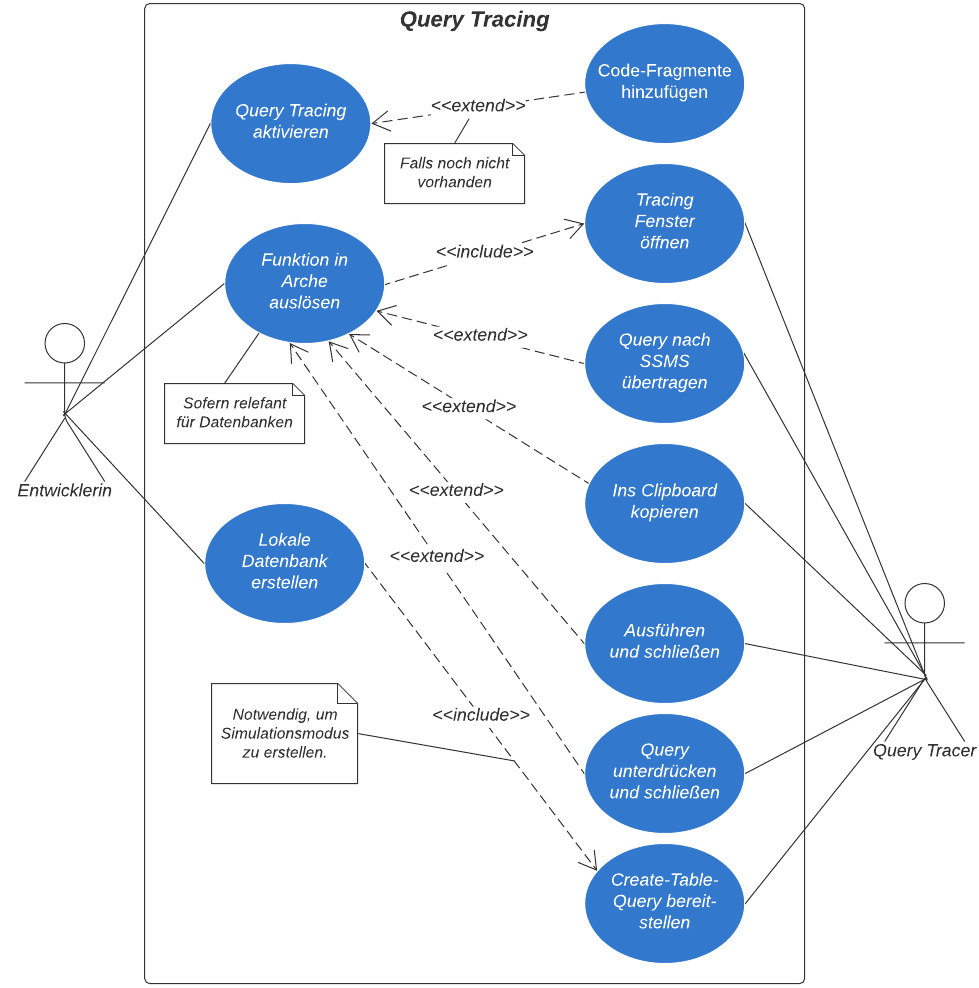
\includegraphics[scale=0.7]{Anwendungsfalldiagramm_2.png}
                    
                    \end{figure}
        \end{frame}
        
        \begin{frame}{Anwendungsfall (2)}
        
            \begin{figure}[htp]
                   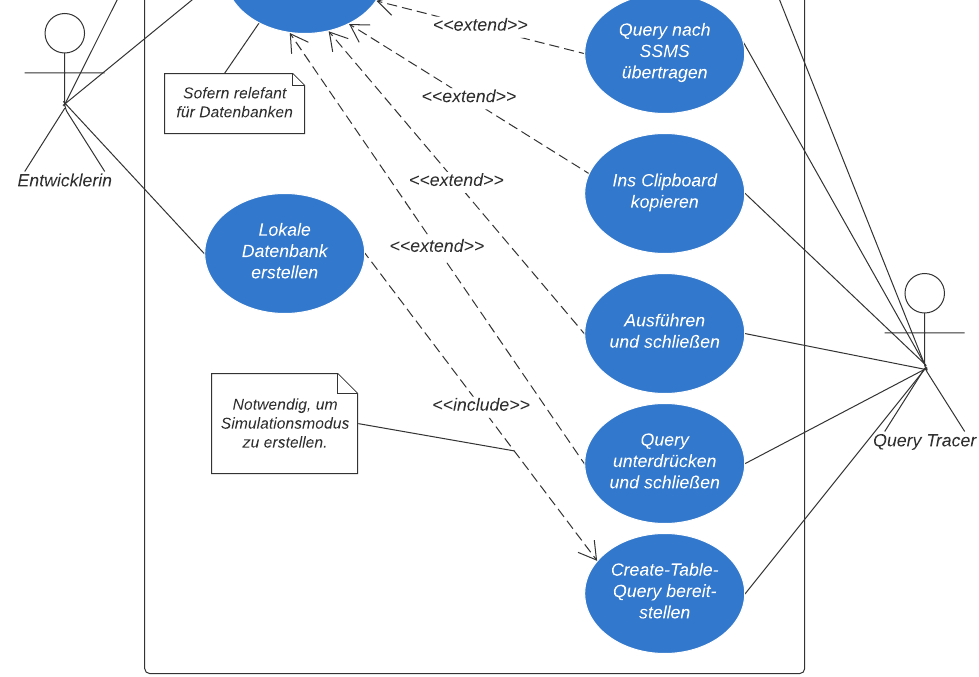
\includegraphics[scale=0.3]{Anwendungsfalldiagramm_2_Crop.png}
                    
                    \end{figure}
        \end{frame}

\end{document}